\section{Ângulo de Dois Vetores}

O ângulo entre dois vetores não nulos \( \overrightarrow{u} \) e \(
\overrightarrow{v} \) é o ângulo \( \theta \) formado pelas semirretas \( OA \)
e \( OB \) com a mesma origem \( O \) (Figura~\ref{fig:fig1.21}), onde \(
\overrightarrow{u} = \overrightarrow{OA} \), \( \overrightarrow{v} =
\overrightarrow{OB} \) e \( 0 \leq \theta \leq \pi \) (em radianos) ou \(
0^\circ \leq \theta \leq 180^\circ \).

\begin{figure}[H]
    \centering
    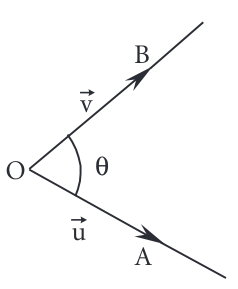
\includegraphics[width=0.3\textwidth]{./fig/fig1.21.png}
    \caption{}\label{fig:fig1.21}
\end{figure}

Se \( \overrightarrow{u} \parallel \overrightarrow{v} \) e possuem o mesmo
sentido, então \( \theta = 0 \), como ocorre com \( \overrightarrow{u} \) e \(
2\overrightarrow{u} \) (Figura~\ref{fig:fig1.22a}).

\begin{figure}[H]
    \centering
    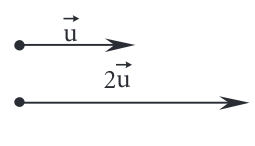
\includegraphics[width=0.5\textwidth]{./fig/fig1.22a.png}
    \caption{}\label{fig:fig1.22a}
\end{figure}

Se \( \overrightarrow{u} \parallel \overrightarrow{v} \) mas possuem sentidos
contrários, então \( \theta = \pi \), como no caso de \( \overrightarrow{u} \) e
\( -3\overrightarrow{u} \) (Figura~\ref{fig:fig1.22b}).

\begin{figure}[H]
    \centering
    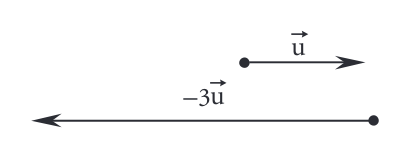
\includegraphics[width=0.5\textwidth]{./fig/fig1.22b.png}
    \caption{}\label{fig:fig1.22b}
\end{figure}
